\documentclass[conference, 10ppt]{IEEEtran}
\usepackage{amsmath,amssymb,amsfonts}
%\usepackage{algorithmic}
\usepackage{graphicx}
\usepackage{textcomp}
\usepackage{xcolor}
\usepackage{comment}
%
%\usepackage{slashbox}
\usepackage{url}
\usepackage{cite}
\usepackage{amsmath,amssymb,amsfonts}
\usepackage{graphicx}
\usepackage{textcomp}
\usepackage{xcolor}
\usepackage{algorithm,algpseudocode}
\algrenewcommand\algorithmicindent{0.9em}%
\usepackage{soul}
\usepackage{xspace}
\usepackage{subfigure}
\usepackage[group-separator={,}, group-minimum-digits=4]{siunitx}
\usepackage{makecell}
\usepackage{multirow}
\usepackage{xcolor,colortbl}

%
\def\BibTeX{{\rm B\kern-.05em{\sc i\kern-.025em b}\kern-.08em
    T\kern-.1667em\lower.7ex\hbox{E}\kern-.125emX}}
 
\begin{document}
%
\newcommand{\todo}[1]{\color{red}\textbf{\hl{#1}}\color{black}\xspace}
%\newcommand{\todo}[1]{}
\newcommand{\rom}[1]{\expandafter{\romannumeral #1\relax}}
%
\title{Performance Model of Iterated SpMV for Distributed System.}

\author{\IEEEauthorblockN{Md Maruf Hossain}
\IEEEauthorblockA{Dept. Computer Science \\
\textit{University of North Carolina at Charlotte}\\
Charlotte, USA \\
mhossa10@uncc.edu}
\and
\IEEEauthorblockN{Erik Saule}
\IEEEauthorblockA{Dept. Computer Science \\
\textit{University of North Carolina at Charlotte}\\
Charlotte, USA \\
esaule@uncc.edu}
}
%
%%
%%
\maketitle
%%

\begin{abstract}
Many applications rely on basic sparse linear algebra operations from numerical solvers to graph analysis 
algorithms. Yet, the performance of these operations is still reasonably unknown. Users and practitioners 
rely on the rule of thumb understanding of what typically works best for some application domain.
\\ 
This paper aims at providing an overall framework for the distributed system to think about the performance 
of sparse applications. We use the sparse matrix-vector(SpMV) multiplication as the representative of the 
experiments. We model the performance of multiple SpMV implementations on distributed systems. 
 We model the performance of different modes of execution of SpMV using linear and polynomial regression models for a distributed system. 
 The models enable us to predict how to partition and represent the sparse matrix to optimize the performance of iterated SpMV on a cluster with 225 cores.
\end{abstract}
%
%%
%%

\begin{IEEEkeywords}
SpMV, MPI, Graph Partitioning
\end{IEEEkeywords}

\section{Introduction}
%%%%%%%%% Why %%%%%%%%%
Sparse matrix-vector multiplication(\textit{SpMV}) is one of the
fundamental operations in sparse linear algebra. It is critical to
solving linear systems and is widely used in engineering and scientific
applications~\cite{gleich2015pagerank, saad2003iterative, dytrych2016efficacy}. 
Distributed memory systems have entered a new age with
the popularization of departmental clusters to support these
scientific and engineering applications.  Many different approaches
have been proposed to improve \textit{SpMV} performance on
clusters. But choosing the right approach still mostly relies on the rule
of thumbs. We posit that building models to predict the performance of
different configurations is the only way to make better-informed
decisions.

In this paper, we propose a linear and polynomial \textit{Support
  Vector Regression}(\textit{SVR})~\cite{awad2015support} model to predict and analyze the
run time of \textit{SpMV} on the distributed system for different ways
to execute the operation. Our system will analyze the predicted run
time and return the best possible algorithm for the system. The
performance of the \textit{SpMV} mainly depends on the size and
structure of the matrices and the architecture of the system. 

%%%%%%%%% How %%%%%%%%
To perform sparse matrix-vector multiplication(\textit{SpMV}) on
distributed systems, the most common mechanism is to partition the
matrix into multiple parts and perform \textit{SpMV} on each part
individually in the different processors. Good partitioning can ensure
better load balance and limits the volume of communication between the
underlying \textit{MPI process}. Many partitioning
algorithms have been proposed to ensure good load balance and to
minimize \textit{MPI communications}~\cite{deveci2015hypergraph, karypis1995multilevel,
  kaya2013analysis}.

%%%%%%%%% What %%%%%%%%
In this paper, we explore two partitioning modes (Uniform
2D-Partitioning and 1D Row Partitioning) and the performance of the
different \textit{SpMV} representation based on these partitioning
mechanisms on distributed systems. We develop a linear and a
polynomial support vector regression (\textit{SVR}) performance models
for SpMV operations on the distributed system for these different
techniques. The models are accurate enough to predict the best
configuration to execute SpMV given a matrix.

\section{Related Work}

There have been lots of previous work have done on the \textit{SpMV}
performance model for the \textit{CPU} and \textit{GPU}
architecture. In particular, Guo and Wang~\cite{guo2013performance}
\textit{et.al.} have proposed a linear model for the general-purpose
\textit{GPU} that can predict the runtime of the \textit{SpMV} based
on the strides size and nonzero per row. There are also some other
\textit{SpMV} models~\cite{nisa2018effective,guo2018performance} that
exist for the \textit{GPU} architectures. A performance model for
\textit{SpMV} on the \textit{GPU} architectures is more common than a
single or distributed system of \textit{CPU} architectures. Consistent
and parallelisms of the \textit{GPU} performance is the main reason
behind this.
model for the GPU. 

\section{SpMV on Distributed Systems}
In \textit{2D-Uniform partitioning},  matrices
are partitioned into both row-wise and column-wise.  There is a choice
in the number of column partitions and row partitions. However, for
iterated SpMV applications, it is common practice to pick a symmetric
partitioning scheme and a number of processors that is a perfect
square. Each MPI process handles one of the portions of the matrix.
Load imbalance is a common issue in 2D partitioning. Many matrices
tend to have a band structure that tends to build very imbalanced
partitioning.  2D-Uniform partitioning can balance the number of rows
and columns but can have a significant load imbalance in the number
of non-zeros in the blocks.

Boman and Devine et al.~\cite{boman2013scalable} noted that
randomizing the order of the matrix can provide good load balance for
SpMV in 2D-Uniform partitioning and is used in scientific
applications~\cite{dytrych2016efficacy}. We adopt this strategy for
our 2D uniform partitioning technique. Each row (and corresponding
vector entry) is assigned to a random process.  Since the expected
number of rows and non-zeros is uniform for all processes, this method
generally achieves a good load balance.

If $P=p^2$ is the number of processes
and $matrix\_size$ is the size of the matrix then each processor
should contain the same
number$\Bigl\lceil\dfrac{matrix\_size}{p}\Bigr\rceil$ of rows and
columns. The last block can be padded with zeros to make blocks of the name size.

With 2D-Uniform partitioning, the execution of the iterated SpMV is
done using the classic methods. Each process performs its local
multiplication. The values are then reduced within each row onto the
diagonal process. These reduced values are then broadcast along with the
column processes for the next iteration of the calculation.

In \textit{1D-Row Partitioning}, matrices are split into row-wise
only. Balancing the load between the processors and minimizing the
communication boils down to solving a K-way graph partitioning
problem~\cite{kaya2013analysis}.  We can define the ID-Row(K-way)
partitioning for a graph $G=(V,E)$ with $|V|=n$, partition $V$ into
$k$ subsets, $V_1, V_2, \dots, V_k$ such that $V_i \cap V_j=\phi$ for
$i\neq j$, $|V_i| = n/k$, and $\cup_i V_i = V$, and the number of
edges of $E$ whose incident vertices belong to different subsets is
minimized. Each partition will allocate to a different MPI
process. We base the 1D row partitioning technique that we will model
on this strategy and we choose the METIS graph partitioning
tool~\cite{karypis1995multilevel} to provide the precise row
partitioning.

In 1D-Row partitioning, one process contains small portions of rows
and their corresponding columns. To perform SpMV on the 1D-Row
partitioning, a processor can hold either the portion of the \textbf{vector
  elements} corresponding to their row elements or the full vector.
We call the strategy where the process holds the entire vector \textit{Global
  1D-Row SpMV}(G1DR-SpMV). In this strategy, all MPI processes
perform matrix multiplication locally on the part of the matrix that
belongs to them. After matrix multiplication, an ALL$\_$Gatherv takes
place to share the updated value of the vector.

We call the strategy where a process only holds the portion of the
vector that it needs \textit{Local 1D-Row SpMV}(L1DR-SpMV).  In this
algorithm, initially, a process performs local matrix multiplication
on the non zero elements whose column belong to the local vector.  For
the rest of the non zero elements whose vector elements belong to the
other processes, it retrieves the relevant part of the vector using
communication tailored to each process using standard MPI point to
point communication primitives.

The METIS K-way partitioning technique minimizes the communications
performed by the Local 1D-Row SpMV. Therefore if METIS can partition
the graph well, one would expect the Local 1D-Row to perform very few
communications. However, if the partitioning is not good, the custom
message strategy only saves few communications and the Global 1D-Row
SpMV would benefit from the effectiveness of MPI Collectives. There is
no point in designing a local 2D scheme since the randomized
partitioning ensures there is little saving to be expected from
customized communications.

The local matrix stored by the nodes can be represented in a number of
formats. We picked the two most popular formats: CSR and COO.

\section{Performance Model}
We build up three different SpMV models and investigate their performance on different algorithms and
storage formats.
\begin{enumerate}
\item SpMV Model from Micro-Benchmark.
\item Support Regression Model.
\item Linear Model.
\end{enumerate} 

\subsection{SpMV Model from Micro-Benchmark}
In this model, we predict the runtime of the SPMV based the performance of couple of micro-benchmark of 
a selected computer architecture. Initially, SpMV on the distributed system can be divided into two main parts,
\begin{itemize}
\item Core Calculation: performance of the matrix-vector calculation in a MPI node.
\item MPI Communication: communication runtime among MPI ranks(processes). 
\end{itemize}
\subsubsection{Core Calculation}
We can represent the basic SpMV by $y=y+Val*x$, which requires two floating point operation(multiply and addition). 
So, we can say we need to calculate NNZ(number of non-zeros) times FMA(fused multiply addition) to perform SpMV.
But, first it needs to load the data and SpMV is bound by the memory bandwidth rather than instruction. So, we 
separated the \textit{core calculation} into,
\begin{itemize}
\item Run time for FMA: $L_{FMA}\times NNZ$, where $L_{FMA}$ is the latency of a single FMA and $NNZ$ is number of non-zeros.
\item Memory access latency: $L_{RW}$
\end{itemize} 

\paragraph{Micro Benchmark for \textit{FMA}}
The throughput of SkylakeX is 2 instructions per cycle and the latency of FMA is 4 cycles. So there is a potential 
of pipelinling($2\times 4 = 8$) to get the optimal results. Now, SkylakeX 
has 512-bit register that can give the ability of the vectorization. For 64-bits floating point operation it can give vector 
width 8 and for 32-bits it can give at max vector width 16. To find the peak performance of the FMA and to avoid the 
read-write latency we need to setup the benchmark that datasets can be contained in the register. Now, SkylakeX has 32 
registers. We can populate the pipeline by using sufficient ampunt of work. By varying the 
number of fused-multiply-addition calculation, we can find out the performance limitation. From the information of the 
processors, we can say that 4 cycles required for \textit{FMA} and the throughput of the FMA is 2 instruction per cycle, that means 
we should at least use $4\times 2=8$ instruction at a time to populate the pipeline.
\begin{figure}[hbt!]
	\centering
	\subfigure[Vector Width: 4]{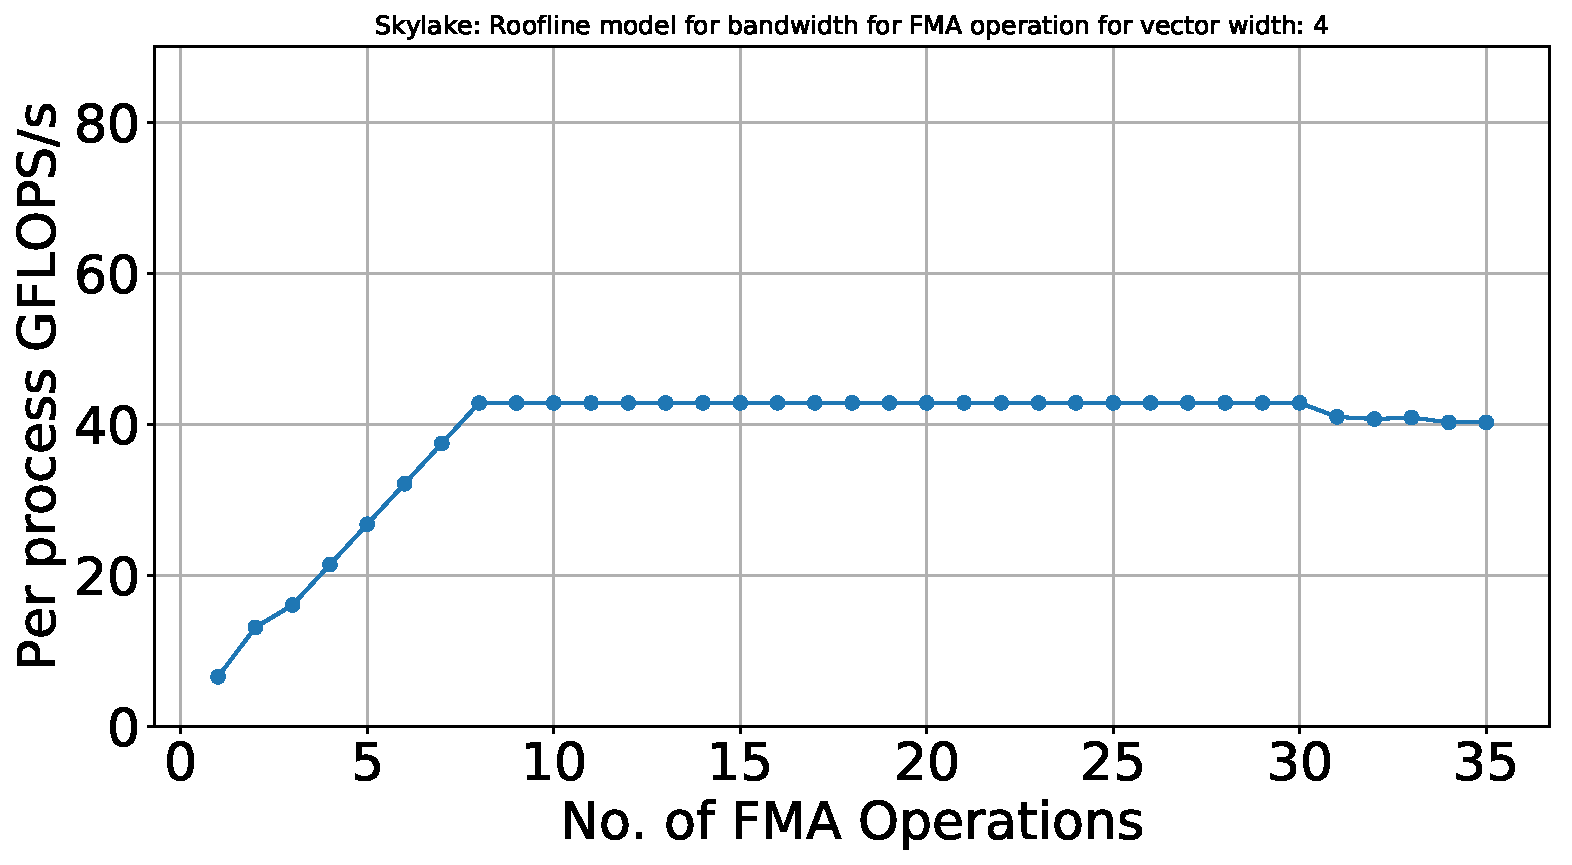
\includegraphics[width=0.48\linewidth]{figures/fma/skylake_mpi_fma_roofline_model_for_vec_4.pdf}		\label{fig:mpi-skl-vec-4}}
	\subfigure[Vector Width: 8]{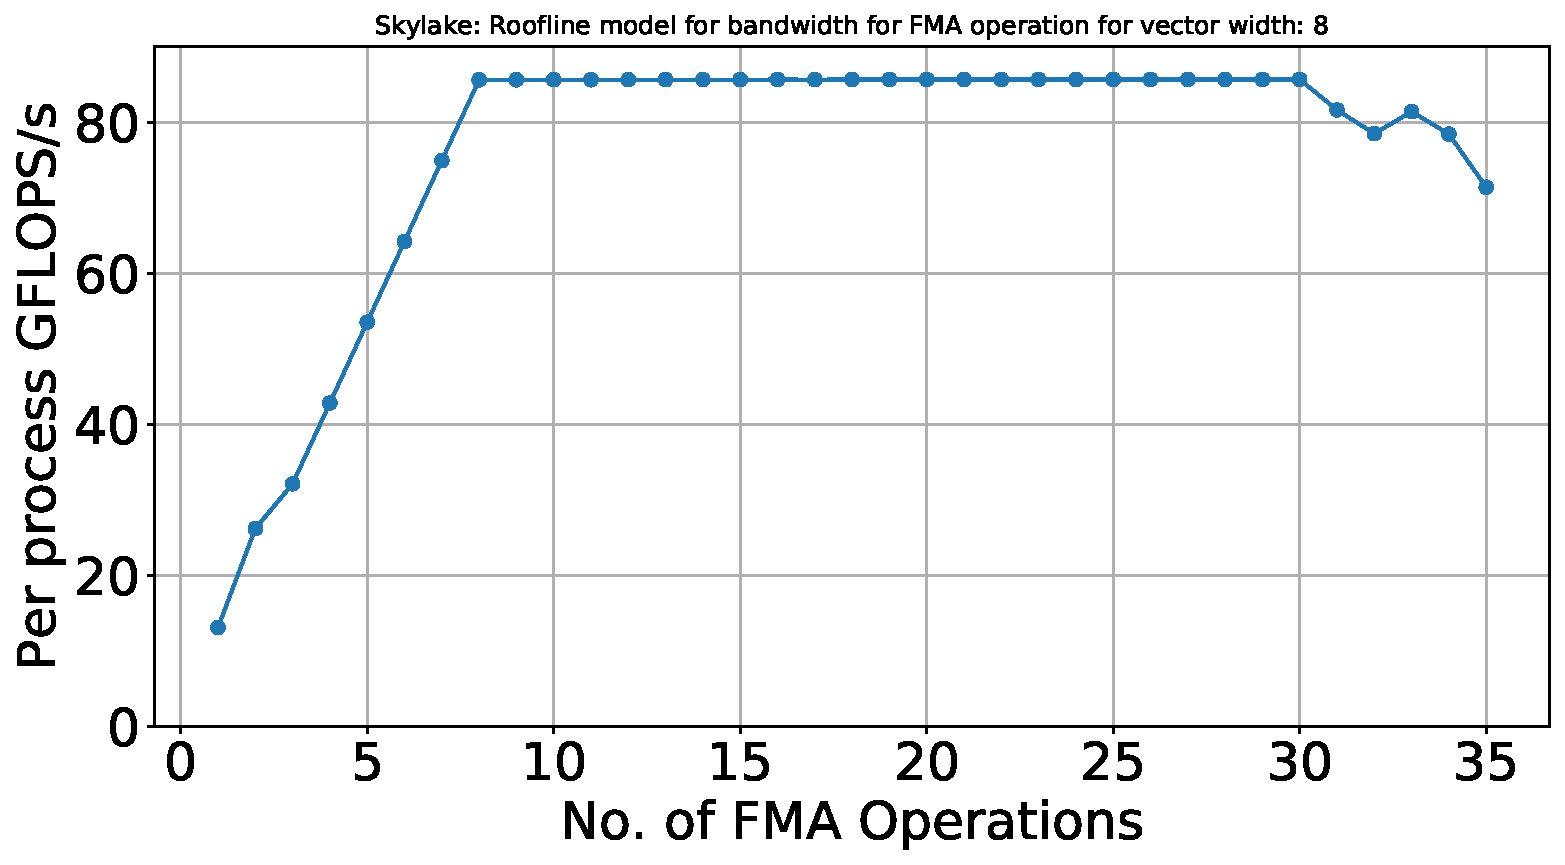
\includegraphics[width=0.48\linewidth]{figures/fma/skylake_mpi_fma_roofline_model_for_vec_8.pdf}		\label{fig:mpi-skl-vec-8}}
	\caption{Skylake: (MPI)Roofline model for bandwidth for FMA operation}
	\label{fig:mpi-skl-fma}
\end{figure}
Figure~\ref{fig:mpi-skl-fma} shows the roofline model of the \textit{FMA} on SkylakeX processor. 
We can estimate the theoritical peak performance a single FMA by the following equation,
\begin{eqnarray*}
P\ =\ Base\_Clock\_Frequency\times Vector\_Width\times \frac{FLOPs}{Instruction}
\end{eqnarray*}
The significance of the \textit{FMA} 
latency is very few compare to the memory access latency. 

\paragraph{Micro-Benchmark for Memory Access Latency}
We explore the \textit{STREAM} benchmark to find out the bandwidth of the memory access for a selected architecture.
\begin{figure}[hbt!]
	\centering
	\subfigure[Single Precision.]{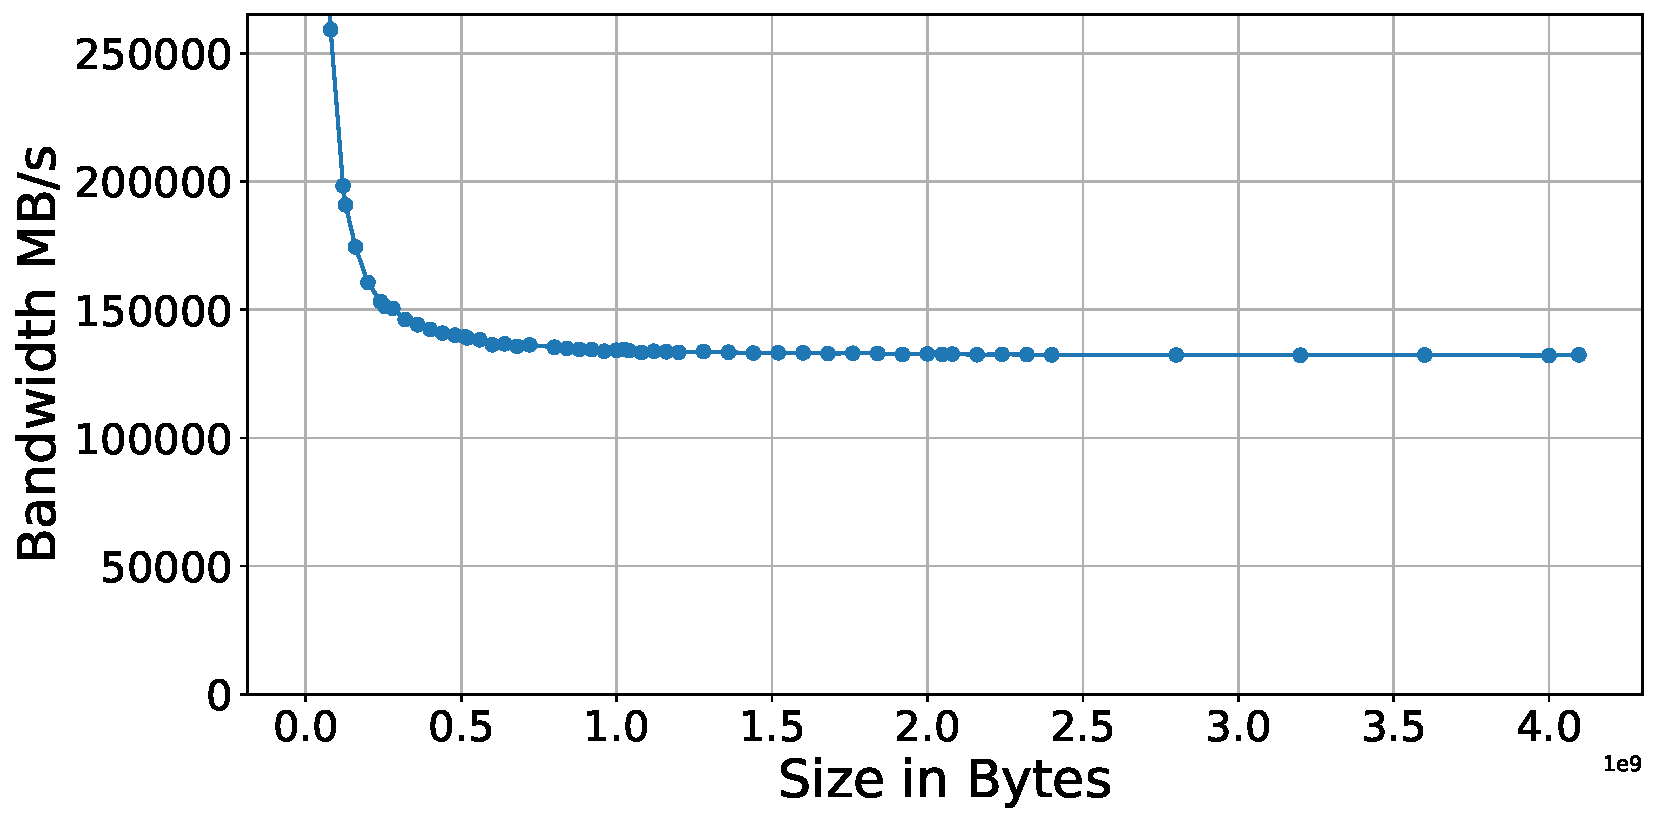
\includegraphics[width=0.48\linewidth]{figures/stream/skylake_mpi_copy_single_precision.pdf}		\label{fig:stream-single-copy}}
	\subfigure[Double Precision.]{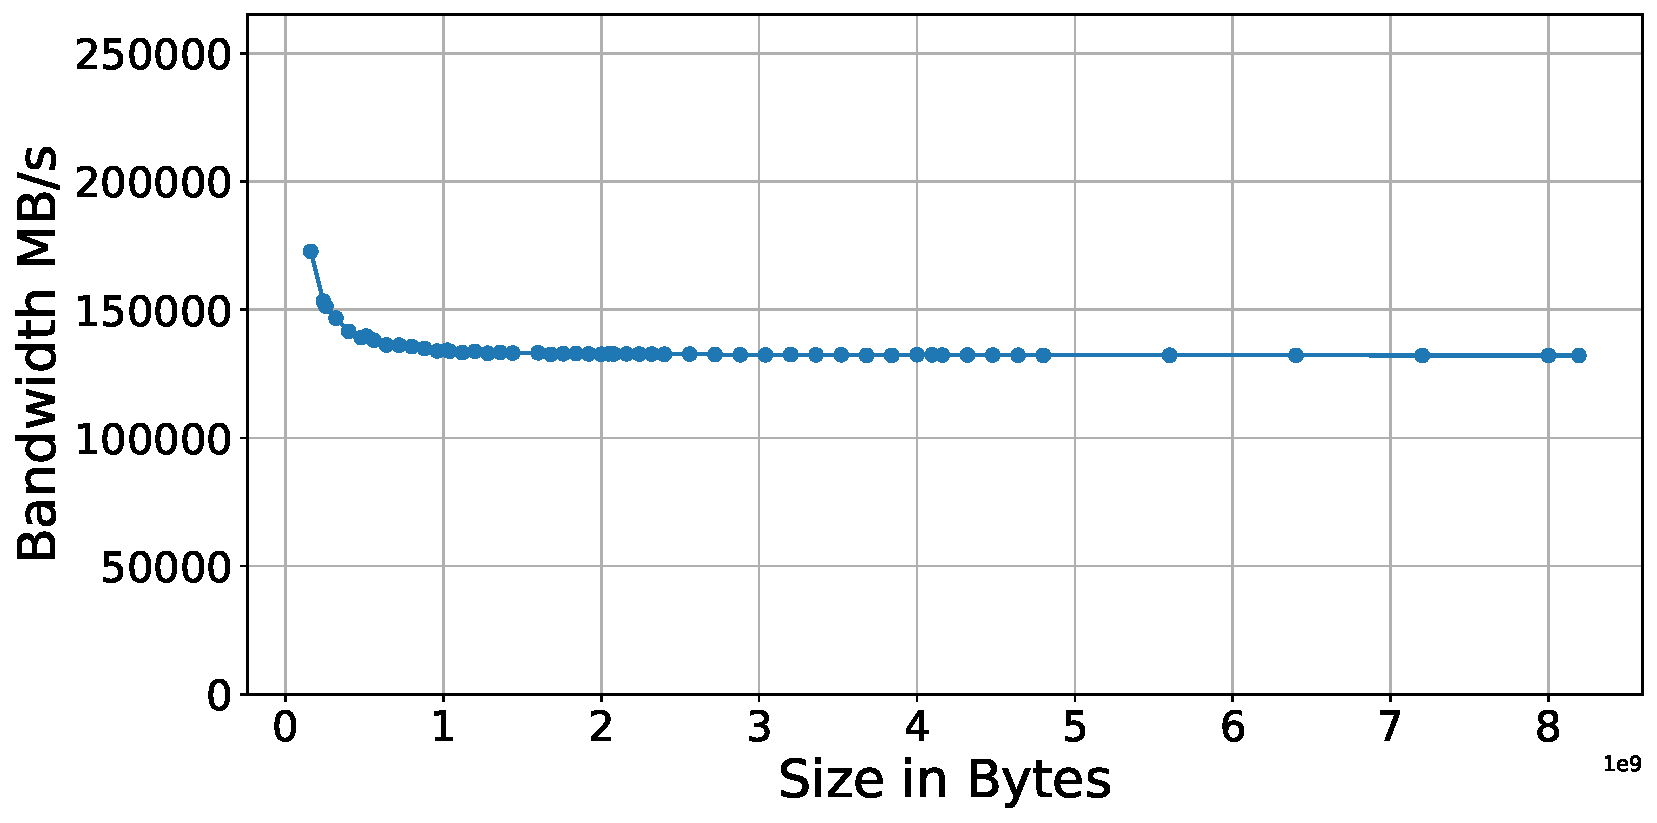
\includegraphics[width=0.48\linewidth]{figures/stream/skylake_mpi_copy_double_precision.pdf}		\label{fig:stream-double-copy}}
	\caption{Single and double precision memory access bandwidth on Skylake processor.}
	\label{fig:stream-copy-bandwidth}
\end{figure}
Figure~\ref{fig:stream-copy-bandwidth} shows the relation between data size and bandwidth of the SkylakeX processor. 
To pick the right bandwidth for a matrix-vector multiplication, we first calculate the size of the data. Based on the size 
of the data, we pick the average of the available immediate lower and higher point of the benchmark. Now, memory can 
be accessed sequentially or random. To calculate the sequential and random access data, we build another micro-benchmark(Cache-Pattern). 
Next, we will discuss about Cache-Pattern benchmark.
 
\paragraph{Cache-Pattern Micro-Benchmark}
In SpMV some array or vector traverse incrementally and some irregular pattern. All the incremental or regular data accesses are treated as 
\textit{Sequential} data. So, we do not need any extra work to handle them. Now, it is not guaranty that all the irregular access pattern data 
are fully random access. There is possibility chunks of data in the middle of the array are sequential. The main aim of this benchmark is to 
separate a irregular access array into sequential and random access data. This benchmark walk through a array and calculate the cache miss 
and hit based on the \textit{least recently used}(LRU) memory. all the \textit{hits} added to the sequential data and \textit{miss} points are 
added to the random access data.
\begin{table}[htb]
\caption{Memory Access Property for 2D-Partitioning SpMV Model(RPP=rows per process, NNZ=non-zero elements).}
\label{tab:csr-spmv-2d-property}
\centering
\begin{tabular}[c]{| l | c | c | c | c | c |}
\hline
\multirow{2}{*}{Array} & \multicolumn{2}{ | c |}{Elements Size} & \multirow{2}{*}{Data Type} & \multicolumn{2}{ | c |}{Access Type} \\ \cline{2-3} \cline{5-6}
  &  CSR & COO  & &  CSR & COO \\ \hline
rowA & 2$\times$RPP & NNZ & Integer & Sequential & Sequential \\ \hline
colA & NNZ & NNZ & Integer & Sequential & Sequential  \\ \hline
valA & NNZ & NNZ & Floating & Sequential &  Sequential \\ \hline
x & NNZ  & NNZ & Floating & Irregular &  Irregular \\ \hline
y & RPP & NNZ & Floating & Sequential & Irregular  \\ \hline
\end{tabular}
\end{table}
Table~\ref{tab:csr-spmv-2d-property} shows the memory access property for the 2D-Partitioning SpMV model. We can see the access 
to the vector \texttt{x} is irregular for both CSR and COO  format. But access to the vector \texttt{y} is only irregular for the COO format. 
But, irregular does not guaranty the fully random access to the memory, that is why we need to separate the \texttt{x} for both and \texttt{y} 
for COO format into \textit{hit} and \textit{miss} portions.  
All the data size is determined for all the MPI ranks of a whole node.

\subsubsection{Micro-Benchmark for MPI communication}
MPI communications mostly depend on the size of the message and network topology. We build a benchmark based on the OSU-MPI-Benchmark.
Because of the dynamics of the network topology we build a polynomial model based on the number of nodes, number of MPI ranks, message size, 
and MPI communication type.  

\begin{comment}
\begin{figure}[hbt!]
	\centering
	\subfigure[MPI All\_GatherV.]{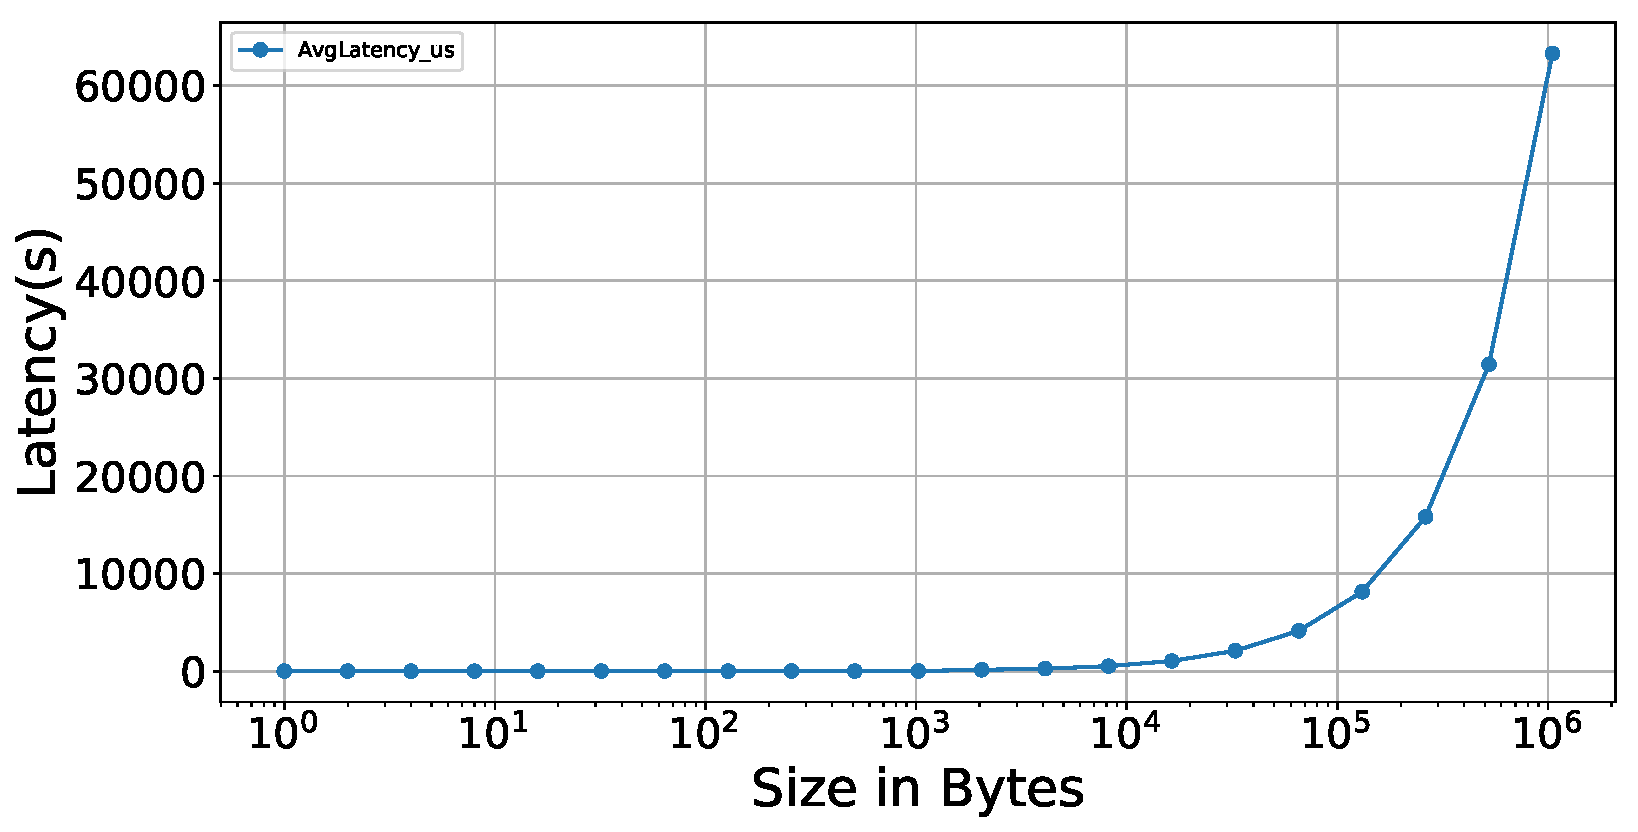
\includegraphics[width=0.48\linewidth]{figures/osu/skylake_mpi_allgatherv.pdf}		\label{fig:osu-skylake-allgatherv}}
	\subfigure[MPI All\_Reduce.]{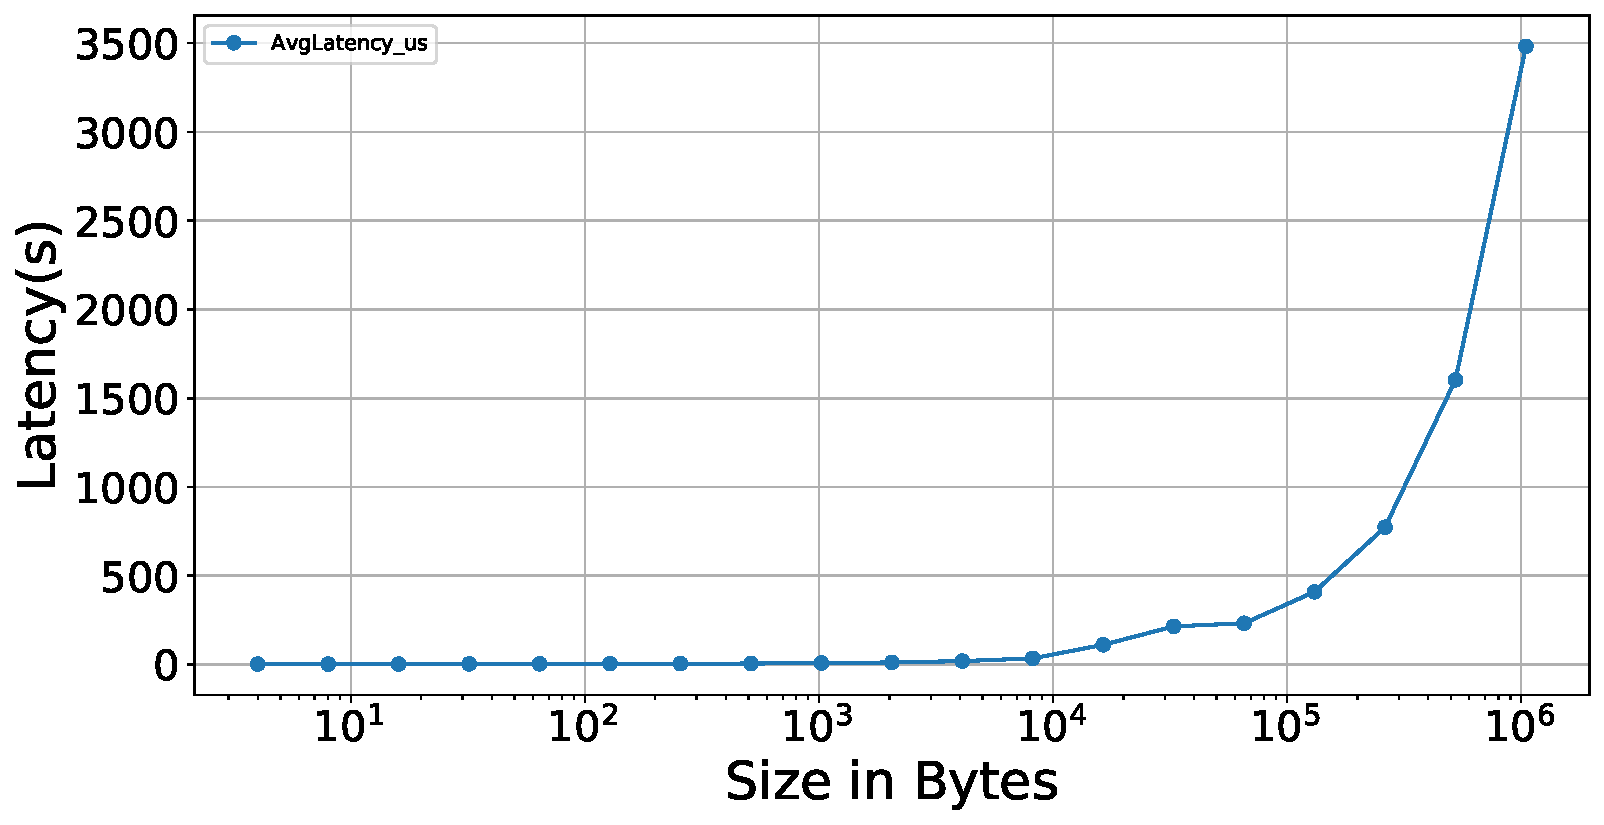
\includegraphics[width=0.48\linewidth]{figures/osu/skylake_mpi_allreduce.pdf}		\label{fig:osu-skylake-reduce}}
	\caption{Latency of the MPI collectives(All\_GatherV and All\_Reduce) on Skylake.}
	\label{fig:osu-collectives}
\end{figure}
\end{comment}

Figure~\ref{fig:spmv-model-from-benchmark} shows the overall structure of the SPMV model from micro-benchmark.

\begin{figure}[hbt!]
	\centering
	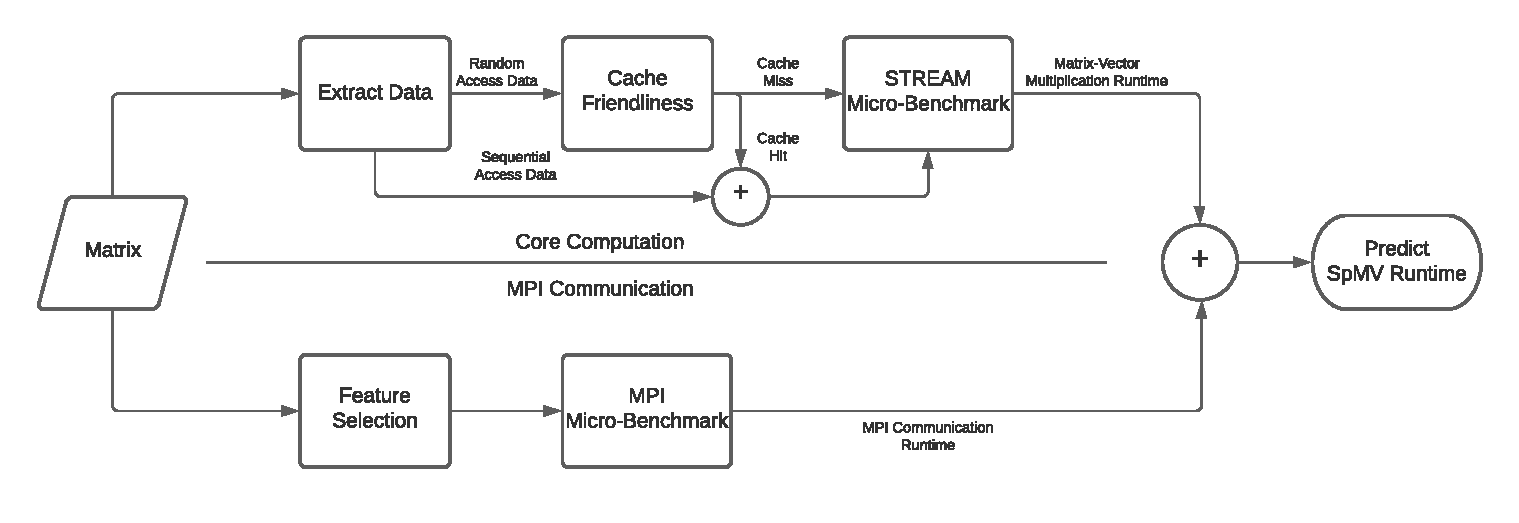
\includegraphics[width=0.96\linewidth]{figures/spmv_hardware_model.pdf}
	\caption{Structure of the SpMV model from micro-benchmark.}
	\label{fig:spmv-model-from-benchmark}
\end{figure}



\subsection{Linear Model}
\label{sec:linear-2d-spmv}
We build up a linear model from generated random matrices of the different
number of rows. For each matrix with specific rows, we generated
matrices with the different number of nonzeros per row $1, 2, 4, 8, 16,
\dots, 128$. Then build a linear regression model for a particular row
size matrix against the nonzeros per row. Our aim to find out two near
similar generated matrix $A$ and $B$ for given test matrix($M$), that
the number rows in $A$ and $B$ immediate lower and higher than $M$
respectively form the available matrices of the model. Then we predict
the performance of the test matrix $M$ based on these two model
matrices.

We realized in early investigations that the linear models would not
perform well on 1D partitioning models because the local number of non
zero varies significantly. However, in the uniform 2D-Partitioning
\textit{SpMV}, every process receives a matrix where non-zero are
distributed randomly.

Figure~\ref{fig:npr} shows the linearity of the run time over the
non-zero per row for a particular matrix. It confirmed that we should
build a regression model that can predict the run time of
\textit{SpMV} based on the non zero per row. We build multiple linear
models using the different sizes of the random matrix. Each model
trains by the different number of non-zeros per row but the same row
size.

If a test matrix has $r$ row and $npr$ non-zero per row, then our
system will find two linear models($L_1, L_2$) for row $r_1$ and $r_2$
like $r_1\leq r\leq r_2$.  It is important to note that, $L_1(r_1)$
and $L_2(r_2)$ are the two models with immediate smaller and larger rows
than $r$ respectively.  The following two equations represent the
linear model $L_1(r_1)$ and $L2(r_2)$,
\begin{equation*}
\begin{array}{l}
y_1\ =\ m_1\times x\ +\ c_1  \qquad\qquad\text{for } r_1 \ \text{and } x=npr\\
y_2\ =\ m_2\times x\ +\ c_2  \qquad\qquad\text{for } r_2 \ \text{and } x=npr
\end{array}
\end{equation*}

According to our model, we expect the performance($y$) of the subject
matrix with row $r$ is between $y_1$ and $y_2$ ($y_1\leq y\leq
y_2$). Our system finally predict the execution run time of the
subject matrix using the following equation,

\begin{equation*}
\begin{array}{l}
y\ =\ y_1+\frac{(y_2-y_1) (r-r_1)}{r_2-r_1}
\end{array}
\end{equation*}
\begin{figure}[hbt!]
\centering
\subfigure[Nonzer per row vs run time for different matrices.]{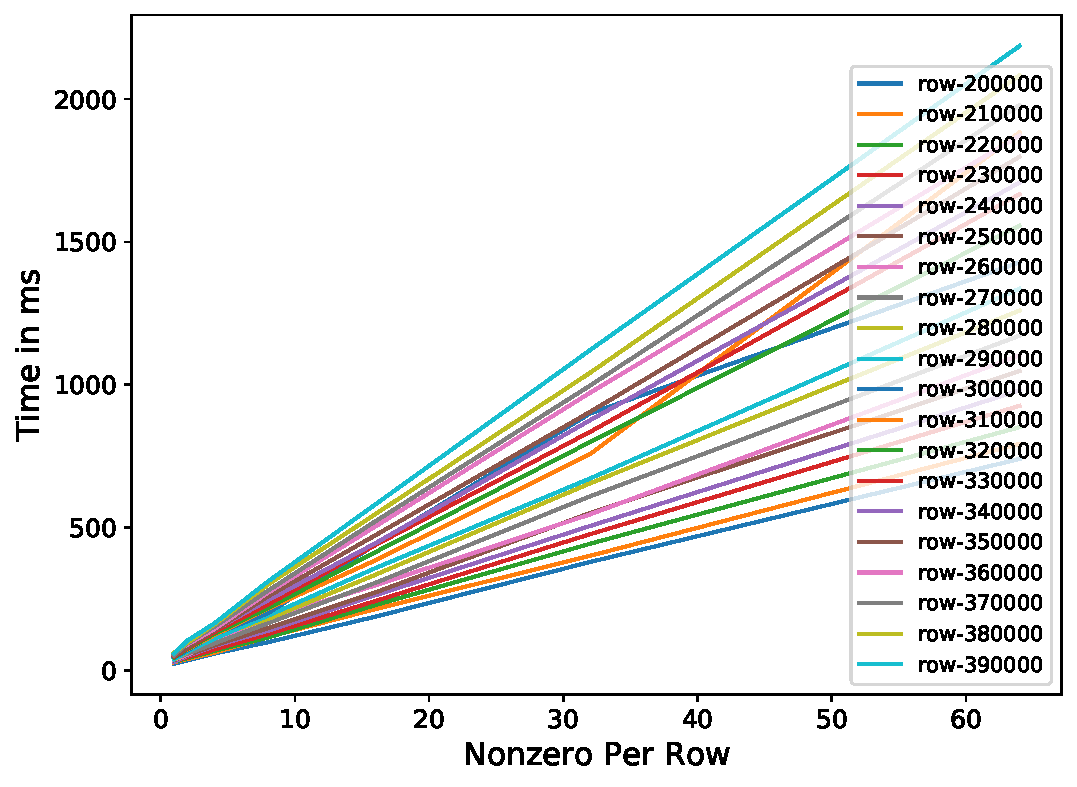
\includegraphics[width=0.48\linewidth]{figures/model_nonzero_perRow_for_particular_row_process_100.pdf}\label{fig:npr}}
\subfigure[Sample equation for the linear model.]{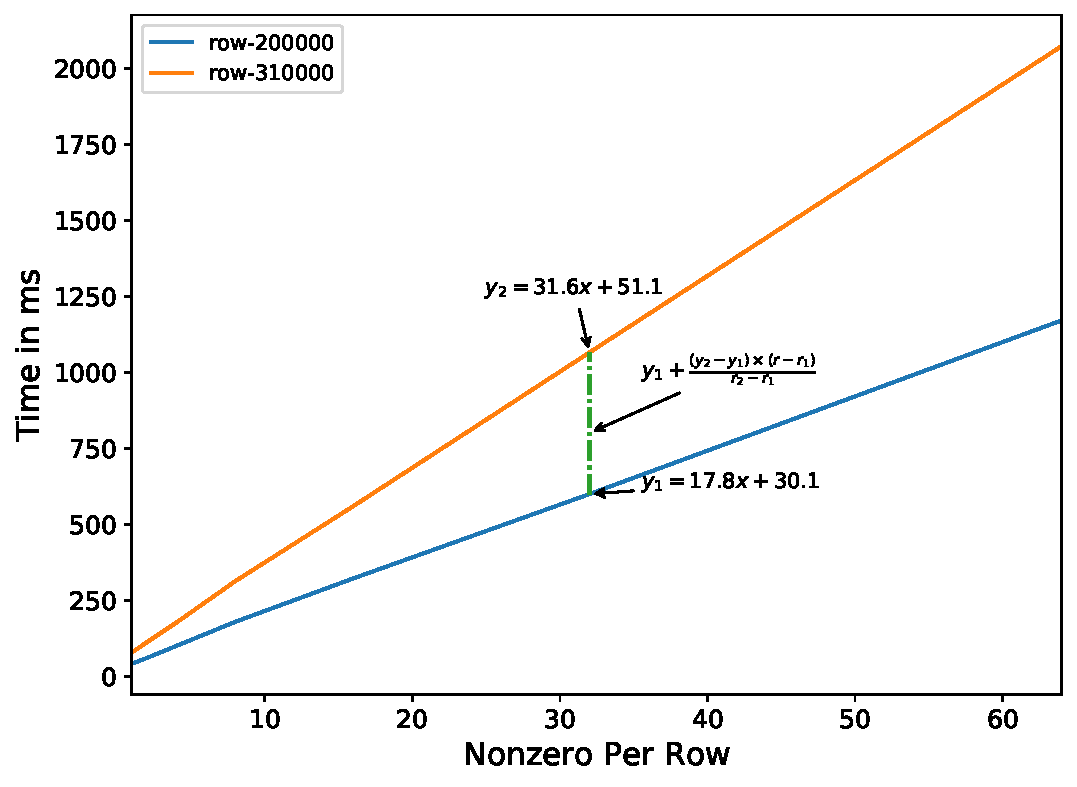
\includegraphics[width=0.48\linewidth]{figures/prediction_equation.pdf}\label{fig:linearspmvmodel}}
\caption{Linear relationship between nonzero per row and run time for the SpMV on the uniform 2d-Partitioning.}
\label{fig:ov-linear-model}
\end{figure}
Figure~\ref{fig:linearspmvmodel} shows the example for the matrix with $250000$ average rows per process and 32 nonzero per row. 
Here, possible $r_1$ and $r_2$ equations are available for rows $200000$ and $310000$. The figure reflects the prediction mechanism of our 
system. 


\subsection{Polynomial Support Vector Regression(SVR) Model}
\label{sec:svr-spmv}
We build the polynomial SVR model for all three algorithms
(\textit{2D-Uniform partitioning SpMV, G1DR-SpMV, and L1DR-SpMV}). The
performance of the SVR models largely depends on the appropriate
attributes for the model. Then choose the proper values for the
\textit{free parameters} of the SVR model.  \textit{Cross-Validation}
and \textit{Grid-Search} widely use to do that for the SVR model. The
models are built for a particular system, therefore they assume a
fixed number of processors and interconnect.

\subsubsection{Cross-Validation and Grid-Search}
Initially, we split the matrices into train and test data set, no test
data participate in the training mechanism. Here, we choose the
polynomial (``poly'') kernel to perform all the machine learning
regression. In this kernel, some free variables need to choose. 
There are no fixed values for these variables, based on the
application criteria it can vary. We select $5-fold$ cross-validation
that means we split the training set into 5 different parts, and among
5 parts we choose 4 as a training set and the remaining one as a test
set. In the grid search, one need to select a set of variables for the
free variable($C,\gamma$), like $C=\{2^{-2},
2^{-1}, \dots, 2^4, 2^5\}\text{ and }\gamma=\{0.01, 0.02, \dots, 0.2, 0.3\}$
and for each pair of variable need to perform cross-validation and
record the score. Then select a pair that gives the best performance
in cross-validation.  The next step is to train the model using the best
variable on the whole train set.

\subsubsection{Feature selection}
We build up polynomial support vector regression(SVR) models for three
different SpMV algorithms on the two different graph formats(CSR,
COO).  The SVR model follows the same mechanism for all multiplication
algorithm. The model predicts the average run time for a particular
test matrix based on its attributes. So, attributes are the key to a
good performance model.  Although the local multiplication is the same
for every algorithm, the communications are different for the
different partitioning modes. The common attributes for all three
algorithms are:

\begin{enumerate}
\label{list:static-attributes}
\item Average rows per process.
\item Average non zero per process.
\item Average non-zero per row.
\item Density of the matrix.
\item Standard deviation of the non zero per row.
\end{enumerate}

But the communication among the MPI process in the Local L1DR-SpMV
(one-to-one) is different than the other two(one-to-all or all-to-all).
That is why based on the sparsity of the matrices the communication
can vary a lot. For that, we need the following extra attributes for
the L1DR-SpMV which can be extracted after partitioning.

\begin{enumerate}
\item Average local non-zero elements.
\item Average global non-zero elements.
\item Average inter-process call.
\item Average data transfer.
\end{enumerate}

\section{Experimental Settings}
\subsection{Hardware Platform and Operating System}
All the nodes of the computing cluster come with Intel Xeon Gold
6154 processors (SkylakeX architecture) and 388GB of DDR4
memory. Each node has 36 cores in 2 sockets. Hyper-threading is
disabled. The base frequency of each processor is 3.00 GHz.  Each
processor has 25 MB of L3 Cache. The nodes are connected by EDR
Infiniband. The machine uses the \texttt{Linux}. To present
concise results all experiments are performed on 144, 169, 225 and 256 MPI processes
allocated on 4, 5, 7 and 8 nodes respectively. The system support maximum 256 MPI processes.

\subsection{Metrices}
We collect over 90 matrices from the \textit{Florida Sparse Matrix} suit 
and perform train and test on these matrices. We separate test matrices 
to show the test result and the remaining matrices used for the train purpose. 
No test matrices participate in the train process, that is how we make the 
fair test performance. The performance of the machine learning model depend 
on the range of the training sets. That is why we select the test matrices 
that way that they are not out of the range of the train data sets. 

\section{Experimental Results}
\subsection{SpMV Model from Micro-Benchmark}
\subsubsection{Random 2D-SpMV}
Table~\ref{tab:overall-spmv-csr-2d-single} and~\ref{tab:overall-spmv-coo-2d-single} shows the overall performance of the 
SpMV on the 2D-Partitioning model on CSR and COO storage formats respectively.  Average error for the CSR and COO formats are 
$7.62$ and $9.16$ respectively. The error is calculate by,
\begin{eqnarray*}
error =\ \frac{actual\ time - predicted\ time}{actual\ time}\times 100
\end{eqnarray*}
\begin{table}[htb]
\caption{Overall SpMV on Random CSR 2D Partitioning(on Skylake).}
\label{tab:overall-spmv-csr-2d-single}
\centering
\begin{tabular}[c]{| l | c | c | c | c | c |}
\hline
\multirow{2}{*}{Matrices} & \multirow{2}{*}{Nodes} & \multirow{2}{*}{Processes} & \multicolumn{2}{| c |}{Time(s)} & \multirow{2}{*}{Error\%} \\ \cline{4-5}
  &  &  & Actual & Predicted &  \\ \hline
\multirow{4}{*}{333SP}   &  4  &  144  &  7.2E-03  &  7.5E-03  &  4.1\% \\ \cline{2-6}
  &  5  &  169  &  5.7E-03  &  6.6E-03  &  15.1\% \\ \cline{2-6}
  &  7  &  225  &  4.7E-03  &  5.2E-03  &  8.8\% \\ \cline{2-6}
  &  8  &  256  &  4.2E-03  &  4.5E-03  &  6.1\% \\ \hline
\multirow{4}{*}{AS365}  &  4  &  144  &  7.4E-03  &  7.8E-03  &  4.7\% \\ \cline{2-6}
  &  5  &  169  &  5.8E-03  &  6.8E-03  &  15.8\% \\ \cline{2-6}
  &  7  &  225  &  4.7E-03  &  5.3E-03  &  13.5\% \\ \cline{2-6}
  &  8  &  256  &  4.4E-03  &  4.6E-03  &  6.1\% \\ \hline
\multirow{4}{*}{M6}   &  4  &  144  &  6.8E-03  &  7.0E-03  &  2.7\% \\ \cline{2-6}
  &  5  &  169  &  5.3E-03  &  6.1E-03  &  15.0\% \\ \cline{2-6}
  &  7  &  225  &  4.4E-03  &  4.8E-03  &  9.4\% \\ \cline{2-6}
  &  8  &  256  &  4.0E-03  &  4.2E-03  &  4.7\% \\ \hline
\multirow{4}{*}{NLR}   &  4  &  144  &  8.2E-03  &  8.7E-03  &  6.3\% \\ \cline{2-6}
  &  5  &  169  &  6.5E-03  &  7.6E-03  &  17.8\% \\ \cline{2-6}
  &  7  &  225  &  5.4E-03  &  6.0E-03  &  10.9\% \\ \cline{2-6}
  &  8  &  256  &  4.8E-03  &  5.2E-03  &  9.0\% \\ \hline
\multirow{4}{*}{hugetrace-00010}  &  4  &  144  &  2.3E-02  &  2.2E-02  &  2.9\% \\ \cline{2-6}
  &  5  &  169  &  2.0E-02  &  2.0E-02  &  1.6\% \\ \cline{2-6}
  &  7  &  225  &  1.7E-02  &  1.6E-02  &  5.6\% \\ \cline{2-6}
  &  8  &  256  &  1.4E-02  &  1.5E-02  &  8.6\% \\ \hline
\multirow{4}{*}{road\_central}  &  4  &  144  &  2.5E-02  &  2.4E-02  &  2.5\% \\ \cline{2-6}
  &  5  &  169  &  2.2E-02  &  2.2E-02  &  1.4\% \\ \cline{2-6}
  &  7  &  225  &  1.9E-02  &  1.8E-02  &  5.2\% \\ \cline{2-6}
  &  8  &  256  &  1.5E-02  &  1.6E-02  &  7.2\% \\ \hline
\multirow{4}{*}{road\_usa}  &  4  &  144  &  3.6E-02  &  4.1E-02  &  15.0\% \\ \cline{2-6}
  &  5  &  169  &  3.6E-02  &  3.8E-02  &  5.2\% \\ \cline{2-6}
  &  7  &  225  &  3.1E-02  &  3.1E-02  &  1.6\% \\ \cline{2-6}
\  &  8  &  256  &  2.7E-02  &  2.8E-02  &  6.6\% \\ \hline
\end{tabular}
\end{table}

\begin{table}[htb]
\caption{Overall SpMV on Random COO 2D Partitioning(on Skylake).}
\label{tab:overall-spmv-coo-2d-single}
\centering
\begin{tabular}[c]{| l | c | c | c | c | c |}
\hline
\multirow{2}{*}{Matrices} & \multirow{2}{*}{Nodes} & \multirow{2}{*}{Processes} & \multicolumn{2}{| c |}{Time(s)} & \multirow{2}{*}{Error\%} \\ \cline{4-5}
  &  &  & Actual & Predicted &  \\ \hline
\multirow{4}{*}{333SP}   &  4  &  144  &  5.4E-03  &  5.6E-03  &  3.7\% \\ \cline{2-6}
  &  5  &  169  &  4.2E-03  &  5.0E-03  &  19.6\% \\ \cline{2-6}
  &  7  &  225  &  3.5E-03  &  4.0E-03  &  15.5\% \\ \cline{2-6}
  &  8  &  256  &  3.4E-03  &  3.5E-03  &  4.3\% \\ \hline
\multirow{4}{*}{AS365}  &  4  &  144  &  5.5E-03  &  5.8E-03  &  4.0\% \\ \cline{2-6}
  &  5  &  169  &  4.3E-03  &  5.1E-03  &  19.7\% \\ \cline{2-6}
  &  7  &  225  &  3.6E-03  &  4.1E-03  &  13.6\% \\ \cline{2-6}
  &  8  &  256  &  3.6E-03  &  3.6E-03  &  0.1\% \\ \hline
\multirow{4}{*}{M6}  &  4  &  144  &  5.0E-03  &  5.2E-03  &  3.5\% \\ \cline{2-6}
  &  5  &  169  &  3.9E-03  &  4.6E-03  &  18.7\% \\ \cline{2-6}
  &  7  &  225  &  3.4E-03  &  3.8E-03  &  9.7\% \\ \cline{2-6}
  &  8  &  256  &  3.3E-03  &  3.3E-03  &  0.8\% \\ \hline
\multirow{4}{*}{NLR}  &  4  &  144  &  6.1E-03  &  6.4E-03  &  4.9\% \\ \cline{2-6}
  &  5  &  169  &  4.8E-03  &  5.7E-03  &  19.6\% \\ \cline{2-6}
  &  7  &  225  &  4.0E-03  &  4.6E-03  &  15.2\% \\ \cline{2-6}
  &  8  &  256  &  3.9E-03  &  4.0E-03  &  2.8\% \\ \hline
\multirow{4}{*}{hugetrace-00010}   &  4  &  144  &  1.7E-02  &  1.6E-02  &  4.2\% \\ \cline{2-6}
  &  5  &  169  &  1.3E-02  &  1.5E-02  &  13.7\% \\ \cline{2-6}
  &  7  &  225  &  1.1E-02  &  1.2E-02  &  9.5\% \\ \cline{2-6}
  &  8  &  256  &  1.0E-02  &  1.1E-02  &  9.2\% \\ \hline
\multirow{4}{*}{road\_central}  &  4  &  144  &  1.9E-02  &  1.8E-02  &  5.6\% \\ \cline{2-6}
  &  5  &  169  &  1.5E-02  &  1.7E-02  &  12.4\% \\ \cline{2-6}
  &  7  &  225  &  1.3E-02  &  1.4E-02  &  8.7\% \\ \cline{2-6}
\  &  8  &  256  &  1.2E-02  &  1.3E-02  &  8.1\% \\ \hline
\multirow{4}{*}{road\_usa}  &  4  &  144  &  2.9E-02  &  3.0E-02  &  3.7\% \\ \cline{2-6}
  &  5  &  169  &  3.2E-02  &  2.8E-02  &  12.6\% \\ \cline{2-6}
  &  7  &  225  &  2.3E-02  &  2.4E-02  &  5.4\% \\ \cline{2-6}
  &  8  &  256  &  2.0E-02  &  2.2E-02  &  7.6\% \\ \hline
\end{tabular}
\end{table}

\subsubsection{Local 1D-SpMV}
Table~\ref{tab:overall-spmv-csr-lk-single} and~\ref{tab:overall-spmv-coo-lk-single} shows the overall performance of the Local 1D-Partitioning 
SpMV model on CSR and COO storage formats respectively.  Average error for the CSR and COO formats are 
$7.31$ and $8.81$ respectively. 

\begin{table}[htb]
\caption{Overall SpMV on Local CSR 1D-Row Partitioning(on Skylake).}
\label{tab:overall-spmv-csr-lk-single}
\centering
\begin{tabular}[c]{| l | c | c | c | c | c |}
\hline
\multirow{2}{*}{Matrices} & \multirow{2}{*}{Nodes} & \multirow{2}{*}{Processes} & \multicolumn{2}{| c |}{Time(s)} & \multirow{2}{*}{Error\%} \\ \cline{4-5}
  &  &  & Actual & Predicted &  \\ \hline
\multirow{4}{*}{333SP}   &  4  &  144  &  1.2E-03  &  1.3E-03  &  9.8\% \\ \cline{2-6}
  &  5  &  169  &  1.1E-03  &  1.2E-03  &  12.6\% \\ \cline{2-6}
  &  7  &  225  &  8.4E-04  &  9.7E-04  &  15.6\% \\ \cline{2-6}
  &  8  &  256  &  8.2E-04  &  8.8E-04  &  6.6\% \\ \hline
\multirow{4}{*}{AS365}  &  4  &  144  &  1.3E-03  &  1.5E-03  &  9.1\% \\ \cline{2-6}
  &  5  &  169  &  1.2E-03  &  1.3E-03  &  10.9\% \\ \cline{2-6}
  &  7  &  225  &  9.3E-04  &  1.0E-03  &  11.5\% \\ \cline{2-6}
  &  8  &  256  &  8.6E-04  &  9.3E-04  &  7.9\% \\ \hline
\multirow{4}{*}{M6}  &  4  &  144  &  1.2E-03  &  1.4E-03  &  12.5\% \\ \cline{2-6}
  &  5  &  169  &  1.1E-03  &  1.2E-03  &  15.4\% \\ \cline{2-6}
  &  7  &  225  &  8.9E-04  &  9.8E-04  &  10.7\% \\ \cline{2-6}
  &  8  &  256  &  8.1E-04  &  8.9E-04  &  9.3\% \\ \hline
\multirow{4}{*}{NLR}  &  4  &  144  &  1.4E-03  &  1.6E-03  &  9.3\% \\ \cline{2-6}
  &  5  &  169  &  1.3E-03  &  1.4E-03  &  8.9\% \\ \cline{2-6}
  &  7  &  225  &  9.8E-04  &  1.1E-03  &  12.0\% \\ \cline{2-6}
  &  8  &  256  &  9.6E-04  &  9.9E-04  &  3.0\% \\ \hline
\multirow{4}{*}{hugetrace-00010}   &  4  &  144  &  2.5E-03  &  2.7E-03  &  5.3\% \\ \cline{2-6}
 &  5  &  169  &  2.2E-03  &  2.4E-03  &  8.8\% \\ \cline{2-6}
 &  7  &  225  &  1.8E-03  &  1.9E-03  &  6.8\% \\ \cline{2-6}
  &  8  &  256  &  1.7E-03  &  1.7E-03  &  2.6\% \\ \hline
\multirow{4}{*}{road\_central}  &  4  &  144  &  2.7E-03  &  2.6E-03  &  2.1\% \\ \cline{2-6}
  &  5  &  169  &  2.4E-03  &  2.3E-03  &  1.5\% \\ \cline{2-6}
  &  7  &  225  &  1.9E-03  &  1.9E-03  &  0.5\% \\ \cline{2-6}
  &  8  &  256  &  1.8E-03  &  1.7E-03  &  1.2\% \\ \hline
\multirow{4}{*}{road\_usa}  &  4  &  144  &  4.1E-03  &  3.8E-03  &  7.9\% \\ \cline{2-6}
  &  5  &  169  &  3.4E-03  &  3.4E-03  &  0.7\% \\ \cline{2-6}
  &  7  &  225  &  2.8E-03  &  2.8E-03  &  1.4\% \\ \cline{2-6}
  &  8  &  256  &  2.6E-03  &  2.6E-03  &  0.7\% \\ \hline
\end{tabular}
\end{table}

\begin{table}[htb]
\caption{Overall SpMV on Local COO 1D-Row Partitioning(on Skylake).}
\label{tab:overall-spmv-coo-lk-single}
\centering
\begin{tabular}[c]{| l | c | c | c | c | c |}
\hline
\multirow{2}{*}{Matrices} & \multirow{2}{*}{Nodes} & \multirow{2}{*}{Processes} & \multicolumn{2}{| c |}{Time(s)} & \multirow{2}{*}{Error\%} \\ \cline{4-5}
  &  &  & Actual & Predicted &  \\ \hline
\multirow{4}{*}{333SP}  &  4  &  144  &  1.2E-03  &  1.1E-03  &  8.6\% \\ \cline{2-6}
 &  5  &  169  &  1.1E-03  &  9.6E-04  &  11.8\% \\ \cline{2-6}
 &  7  &  225  &  8.9E-04  &  8.2E-04  &  8.7\% \\ \cline{2-6}
 &  8  &  256  &  8.2E-04  &  7.8E-04  &  5.6\% \\ \hline
\multirow{4}{*}{AS365}  &  4  &  144  &  1.4E-03  &  1.2E-03  &  11.0\% \\ \cline{2-6}
 &  5  &  169  &  1.2E-03  &  1.1E-03  &  7.0\% \\ \cline{2-6}
 &  7  &  225  &  9.3E-04  &  9.1E-04  &  2.4\% \\ \cline{2-6}
 &  8  &  256  &  8.5E-04  &  8.7E-04  &  2.9\% \\ \hline
\multirow{4}{*}{M6}  &  4  &  144  &  1.3E-03  &  1.2E-03  &  6.9\% \\ \cline{2-6}
 &  5  &  169  &  1.1E-03  &  1.0E-03  &  8.9\% \\ \cline{2-6}
 &  7  &  225  &  9.1E-04  &  8.7E-04  &  4.5\% \\ \cline{2-6}
 &  8  &  256  &  8.2E-04  &  8.5E-04  &  2.7\% \\ \hline
\multirow{4}{*}{NLR}  &  4  &  144  &  1.4E-03  &  1.3E-03  &  7.8\% \\ \cline{2-6}
 &  5  &  169  &  1.3E-03  &  1.1E-03  &  12.1\% \\ \cline{2-6}
 &  7  &  225  &  1.0E-03  &  9.6E-04  &  5.7\% \\ \cline{2-6}
 &  8  &  256  &  9.6E-04  &  9.2E-04  &  4.4\% \\ \cline{2-6}
\multirow{4}{*}{hugetrace-00010}  &  4  &  144  &  2.5E-03  &  2.2E-03  &  12.3\% \\ \cline{2-6}
 &  5  &  169  &  2.2E-03  &  2.0E-03  &  8.4\% \\ \cline{2-6}
 &  7  &  225  &  1.8E-03  &  1.6E-03  &  6.3\% \\ \cline{2-6}
 &  8  &  256  &  1.6E-03  &  1.5E-03  &  5.1\% \\ \hline
\multirow{4}{*}{road\_central}  &  4  &  144  &  2.5E-03  &  2.1E-03  &  13.0\% \\ \cline{2-6}
 &  5  &  169  &  2.1E-03  &  1.9E-03  &  9.5\% \\ \cline{2-6}
 &  7  &  225  &  1.7E-03  &  1.6E-03  &  7.2\% \\ \cline{2-6}
 &  8  &  256  &  1.6E-03  &  1.5E-03  &  9.2\% \\ \hline
\multirow{4}{*}{road\_usa}  &  4  &  144  &  3.8E-03  &  2.9E-03  &  22.9\% \\ \cline{2-6}
 &  5  &  169  &  3.2E-03  &  2.6E-03  &  18.1\% \\ \cline{2-6}
 &  7  &  225  &  2.6E-03  &  2.2E-03  &  12.2\% \\ \cline{2-6}
 &  8  &  256  &  2.4E-03  &  2.1E-03  &  11.6\% \\ \hline
\end{tabular}
\end{table}


\subsubsection{Local 1D-SpMV}
Table~\ref{tab:overall-spmv-csr-gk-single} and~\ref{tab:overall-spmv-coo-gk-single} shows the overall performance of the Global 1D-Partitioning 
SpMV model on CSR and COO storage formats respectively.  Average error for the CSR and COO formats are 
$13.63$ and $25.3$ respectively. 

\begin{table}[htb]
\caption{Overall SpMV on Global CSR 1D-Row Partitioning(on Skylake).}
\label{tab:overall-spmv-csr-gk-single}
\centering
\begin{tabular}[c]{| l | c | c | c | c | c |}
\hline
\multirow{2}{*}{Matrices} & \multirow{2}{*}{Nodes} & \multirow{2}{*}{Processes} & \multicolumn{2}{| c |}{Time(s)} & \multirow{2}{*}{Error\%} \\ \cline{4-5}
  &  &  & Actual & Predicted &  \\ \hline
\multirow{4}{*}{333SP}  &  4  &  144  &  2.6E-02  &  2.1E-02  &  19.2\% \\ \cline{2-6}
  &  5  &  169  &  2.0E-02  &  2.0E-02  &  2.2\% \\ \cline{2-6}
  &  7  &  225  &  1.9E-02  &  1.8E-02  &  5.6\% \\ \cline{2-6}
  &  8  &  256  &  2.4E-02  &  1.9E-02  &  21.2\% \\ \hline
\multirow{4}{*}{AS365}  &  4  &  144  &  2.7E-02  &  2.2E-02  &  19.2\% \\ \cline{2-6}
  &  5  &  169  &  2.1E-02  &  2.0E-02  &  2.7\% \\ \cline{2-6}
  &  7  &  225  &  2.0E-02  &  1.9E-02  &  4.8\% \\ \cline{2-6}
  &  8  &  256  &  2.4E-02  &  1.9E-02  &  21.3\% \\ \hline
\multirow{4}{*}{M6}   &  4  &  144  &  2.5E-02  &  2.0E-02  &  19.2\% \\ \cline{2-6}
  &  5  &  169  &  1.9E-02  &  1.8E-02  &  3.2\% \\ \cline{2-6}
  &  7  &  225  &  1.8E-02  &  1.7E-02  &  4.5\% \\ \cline{2-6}
  &  8  &  256  &  2.2E-02  &  1.8E-02  &  21.1\% \\ \hline
\multirow{4}{*}{NLR}  &  4  &  144  &  2.9E-02  &  2.4E-02  &  19.2\% \\ \cline{2-6}
  &  5  &  169  &  2.2E-02  &  2.2E-02  &  2.3\% \\ \cline{2-6}
  &  7  &  225  &  2.1E-02  &  2.1E-02  &  4.1\% \\ \cline{2-6}
  &  8  &  256  &  2.6E-02  &  2.1E-02  &  21.3\% \\ \hline
\multirow{4}{*}{hugetrace-00010}  &  4  &  144  &  8.2E-02  &  6.6E-02  &  20.0\% \\ \cline{2-6}
  &  5  &  169  &  6.2E-02  &  6.1E-02  &  0.7\% \\ \cline{2-6}
  &  7  &  225  &  6.4E-02  &  5.7E-02  &  10.2\% \\ \cline{2-6}
  &  8  &  256  &  7.3E-02  &  5.7E-02  &  22.7\% \\ \hline
\multirow{4}{*}{road\_central} &  4  &  144  &  9.6E-02  &  7.6E-02  &  20.2\% \\ \cline{2-6}
\  &  5  &  169  &  7.1E-02  &  7.1E-02  &  0.5\% \\ \cline{2-6}
  &  7  &  225  &  7.4E-02  &  6.6E-02  &  10.3\% \\ \cline{2-6}
  &  8  &  256  &  8.6E-02  &  6.6E-02  &  23.4\% \\ \hline
\multirow{4}{*}{road\_usa}   &  4  &  144  &  1.6E-01  &  1.3E-01  &  19.3\% \\ \cline{2-6}
  &  5  &  169  &  9.9E-02  &  1.2E-01  &  23.8\% \\ \cline{2-6}
  &  7  &  225  &  9.8E-02  &  1.1E-01  &  16.5\% \\ \cline{2-6}
  &  8  &  256  &  1.5E-01  &  1.1E-01  &  23.1\% \\ \hline
\end{tabular}
\end{table}

\begin{table}[htb]
\caption{Overall SpMV on Global COO 1D-Row Partitioning(on Skylake).}
\label{tab:overall-spmv-coo-gk-single}
\centering
\begin{tabular}[c]{| l | c | c | c | c | c |}
\hline
\multirow{2}{*}{Matrices} & \multirow{2}{*}{Nodes} & \multirow{2}{*}{Processes} & \multicolumn{2}{| c |}{Time(s)} & \multirow{2}{*}{Error\%} \\ \cline{4-5}
  &  &  & Actual & Predicted &  \\ \hline
\multirow{4}{*}{333SP}  &  4  &  144  &  3.3E-02  &  2.1E-02  &  34.4\% \\ \cline{2-6}
  &  5  &  169  &  2.7E-02  &  2.0E-02  &  26.0\% \\ \cline{2-6}
  &  7  &  225  &  2.4E-02  &  1.9E-02  &  23.9\% \\ \cline{2-6}
  &  8  &  256  &  2.7E-02  &  1.9E-02  &  30.9\% \\ \hline
\multirow{4}{*}{AS365}  &  4  &  144  &  3.3E-02  &  2.2E-02  &  34.4\% \\ \cline{2-6}
  &  5  &  169  &  2.7E-02  &  2.0E-02  &  26.1\% \\ \cline{2-6}
  &  7  &  225  &  2.5E-02  &  1.9E-02  &  24.3\% \\ \cline{2-6}
  &  8  &  256  &  2.8E-02  &  1.9E-02  &  31.0\% \\ \hline
\multirow{4}{*}{M6}  &  4  &  144  &  3.1E-02  &  2.0E-02  &  35.2\% \\ \cline{2-6}
  &  5  &  169  &  2.5E-02  &  1.9E-02  &  26.1\% \\ \cline{2-6}
  &  7  &  225  &  2.3E-02  &  1.7E-02  &  23.9\% \\ \cline{2-6}
  &  8  &  256  &  2.6E-02  &  1.8E-02  &  30.9\% \\ \hline
\multirow{4}{*}{NLR}   &  4  &  144  &  3.6E-02  &  2.4E-02  &  34.5\% \\ \cline{2-6}
  &  5  &  169  &  3.0E-02  &  2.2E-02  &  26.1\% \\ \cline{2-6}
  &  7  &  225  &  2.7E-02  &  2.1E-02  &  24.1\% \\ \cline{2-6}
  &  8  &  256  &  3.0E-02  &  2.1E-02  &  31.1\% \\ \hline
\multirow{4}{*}{hugetrace-00010}  &  4  &  144  &  9.3E-02  &  6.6E-02  &  28.6\% \\ \cline{2-6}
  &  5  &  169  &  6.7E-02  &  6.2E-02  &  7.6\% \\ \cline{2-6}
  &  7  &  225  &  7.0E-02  &  5.7E-02  &  18.3\% \\ \cline{2-6}
  &  8  &  256  &  7.9E-02  &  5.7E-02  &  28.2\% \\ \hline
\multirow{4}{*}{road\_central}  &  4  &  144  &  1.1E-01  &  7.7E-02  &  27.1\% \\ \cline{2-6}
  &  5  &  169  &  7.1E-02  &  7.2E-02  &  1.7\% \\ \cline{2-6}
  &  7  &  225  &  8.0E-02  &  6.7E-02  &  16.6\% \\ \cline{2-6}
  &  8  &  256  &  9.1E-02  &  6.6E-02  &  27.9\% \\ \hline
\multirow{4}{*}{road\_usa}  &  4  &  144  &  1.8E-01  &  1.3E-01  &  26.1\% \\ \cline{2-6}
  &  5  &  169  &  1.5E-01  &  1.2E-01  &  16.0\% \\ \cline{2-6}
  &  7  &  225  &  1.4E-01  &  1.1E-01  &  20.1\% \\ \cline{2-6}
  &  8  &  256  &  1.5E-01  &  1.1E-01  &  27.4\% \\ \hline
\end{tabular}
\end{table}

\subsection{Polynomial SVR Model}
Table~\ref{tab:dynamic-svr-spmv-performance} shows the performance of the dynamic SVR model for the SpMV 
and the prediction from the polynomial SVR model for two different
graph storage formats on each algorithm. The column \textit{Pred}
represents the predicted run time from the SVR model and the
\textit{Actual} represents the real run time of the SpMV. A green cell of  
Table~\ref{tab:dynamic-svr-spmv-performance}, represents a correct prediction of our
models; while a red cell represents that our models predicted the best
strategy incorrectly and storage format incorrectly. 

The average error for uniform 2D-Partitioning are $9.19$ and $5.27$ for
CSR and COO representation respectively.  The model gives $9.86$ and
$6.55$ average error for the G1DR on CSR and COO format
respectively. The average error for L1DR is $14.15$ for CSR and $13.22$
for the COO storage format.


\section{Conclusion}
In this paper, we provide three SpMV models to predict the run time of the
SpMV on the \textit{Uniform 2D-Partitioning}, \textit{GK-SpMV} and \textit{LK-SpMV}). 
The performance models can predict the run time accurately enough to identify the
optimal strategy to compute SpMV. Our models consider the matrix structure and partitioning information to 
predict the best possible communication strategy to perform
\textit{SpMV}. These models can be useful for the other graph
algorithms that heavily relies on the performance of the SpMV, such as
\textit{page rank}. The model may need to be adjusted to predict the
correct graph representation format.

\begin{table*}
 \caption{Dynamic SVR performance model for SpMV on SkylakeX.}
 \label{tab:dynamic-svr-spmv-performance}
 \centering
 \begin{tabular}[c]{| l | c | c | c | c | c | c | c | c |}
 \hline
\multirow{2}{*}{Name} & \multirow{2}{*}{Nodes} & \multirow{2}{*}{Processes} & \multicolumn{6}{c |} {Error\%} \\ \cline{4-9}
 &  &  & CSR L1DR & COO L1DRV & CSR G1DR & COO G1DR & CSR 2DU & COO 2DU \\ \hline
\multirow{4}{*}{333SP}  &  4  &  144 & \cellcolor{green!25}  15.8 & 15.5 & 3.11 & 2.24 & 0.47 & 5.89 \\ \cline{2-9}
 &  5  &  169 & \cellcolor{green!25}  17.6 & 18.7 & 11.9 & 6.55 & 17.4 & 9.52 \\ \cline{2-9}
 &  7  &  225 & \cellcolor{green!25}  20.3 & 20.9 & 8.65 & 6.21 & 16.5 & 8.79 \\ \cline{2-9}
 &  8  &  256 & \cellcolor{green!25}  24.6 & 22.6 & 5.36 & 3.16 & 13.2 & 2.79 \\ \hline
\multirow{4}{*}{AS365}  &  4  &  144 & \cellcolor{green!25}  20.2 & 19.1 & 2.98 & 2.15 & 0.618 & 5.99 \\ \cline{2-9}
 &  5  &  169 & \cellcolor{green!25}  19.7 & 17.7 & 11.5 & 6.58 & 17.2 & 9.17 \\ \cline{2-9}
 &  7  &  225 & \cellcolor{green!25}  23.2 & 20.0 & 9.61 & 5.71 & 20.6 & 6.52 \\ \cline{2-9}
 &  8  &  256 & \cellcolor{red!25}  22.8 & \cellcolor{blue!25}  18.1 & 5.38 & 3.35 & 12.3 & 1.89 \\ \hline
\multirow{4}{*}{M6}  &  4  &  144 & \cellcolor{green!25}  20.7 & 18.8 & 3.22 & 3.5 & 0.178 & 5.06 \\ \cline{2-9}
 &  5  &  169 & \cellcolor{green!25}  19.0 & 20.4 & 10.6 & 6.44 & 19.8 & 9.95 \\ \cline{2-9}
 &  7  &  225 & \cellcolor{green!25}  23.9 & 23.8 & 9.68 & 6.04 & 19.7 & 4.55 \\ \cline{2-9}
 &  8  &  256 & \cellcolor{red!25}  25.1 & \cellcolor{blue!25}  21.1 & 5.31 & 3.31 & 14.1 & 1.04 \\ \hline
\multirow{4}{*}{NLR}  &  4  &  144 & \cellcolor{green!25}  18.2 & 15.0 & 2.85 & 2.07 & 1.8 & 6.51 \\ \cline{2-9}
 &  5  &  169 & \cellcolor{green!25}  21.2 & 18.9 & 12.2 & 6.81 & 15.9 & 7.37 \\ \cline{2-9}
 &  7  &  225 & \cellcolor{green!25}  22.1 & 19.8 & 10.7 & 6.14 & 14.5 & 6.27 \\ \cline{2-9}
 &  8  &  256 & \cellcolor{green!25}  24.6 & 22.8 & 5.28 & 3.26 & 11.8 & 1.08 \\ \hline
\multirow{4}{*}{hugetrace-00010}  &  4  &  144 & \cellcolor{blue!25}  0.609 & \cellcolor{red!25}  3.1 & 0.732 & 0.784 & 12.2 & 13.4 \\ \cline{2-9}
 &  5  &  169 & \cellcolor{blue!25}  0.358 & \cellcolor{red!25}  2.41 & 18.7 & 25.7 & 6.88 & 2.0 \\ \cline{2-9}
 &  7  &  225 & 6.04 & \cellcolor{green!25}  6.3 & 8.29 & 10.2 & 8.79 & 1.39 \\ \cline{2-9}
 &  8  &  256 & 8.02 & \cellcolor{green!25}  7.71 & 3.33 & 2.02 & 2.43 & 0.431 \\ \hline
\multirow{4}{*}{road\_central}  &  4  &  144 & 2.96 & \cellcolor{green!25}  6.02 & 0.47 & 0.419 & 8.8 & 12.3 \\ \cline{2-9}
 &  5  &  169 & 1.93 & \cellcolor{green!25}  4.52 & 20.9 & 36.4 & 1.11 & 3.44 \\ \cline{2-9}
 &  7  &  225 & 9.17 & \cellcolor{green!25}  0.551 & 8.87 & 11.6 & 5.93 & 0.0307 \\ \cline{2-9}
 &  8  &  256 & 11.0 & \cellcolor{green!25}  3.71 & 3.65 & 2.28 & 3.58 & 1.45 \\ \hline
\multirow{4}{*}{road\_usa}  &  4  &  144 & 3.95 & \cellcolor{green!25}  7.14 & 0.19 & 0.0491 & 7.42 & 1.55 \\ \cline{2-9}
 &  5  &  169 & 5.75 & \cellcolor{green!25}  9.37 & 48.1 & 12.0 & 2.09 & 16.1 \\ \cline{2-9}
 &  7  &  225 & 3.27 & \cellcolor{green!25}  3.87 & 41.0 & 6.56 & 0.00937 & 0.128 \\ \cline{2-9}
 &  8  &  256 & 4.22 & \cellcolor{green!25}  2.11 & 3.34 & 1.79 & 1.98 & 3.05 \\ \hline
  \end{tabular}
\end{table*}


\begin{table*}
\caption{Runtime of SpMV and performance of the SVR model(225 MPI process from Skylake).}
\label{tab:performance_table}
\centering
\begin{tabular}[c]{| l | c | c || c | c || c | c || c | c || c | c || c | c |}
\hline
\multirow{2}{*}{Matrices}  & \multicolumn{2}{c ||} {CSR L1DR}  & \multicolumn{2}{c ||} {COO L1DR}  &  \multicolumn{2}{c ||}{CSR G1DR}  &  \multicolumn{2}{c ||}{COO G1DR}  & \multicolumn{2}{c ||} {CSR 2DU}  &  \multicolumn{2}{c |}{COO 2DU}  \\  \cline{2-13}
 & Actual & Pred & Actual & Pred & Actual & Pred & Actual & Pred & Actual & Pred & Actual & Pred \\ \hline
rmat\_200M2M  &  22.41  &  27.2  &  40.05  &  34.23  &  45.89  &  40.99  &  400.43  &  195.53  &  7.14  &  7.14  &  \textbf{4.73}  & \cellcolor{green!25}  4.7  \\ \hline
rmat\_200M3M  &  27.32  &  30.56  &  29.9  &  34.3  &  39.68  &  45.96  &  243.15  &  288.49  &  8.42  &  9.32  &  \textbf{5.57}  &  \cellcolor{green!25} 5.76  \\ \hline
rmat\_400M4M  &  46.3  &  51.26  &  50.79  &  54.26  &  92.25  &  62.47  &  859.1  &  440.0  &  16.4  &  15.49  &  \textbf{13.91}  &  \cellcolor{green!25} 10.94  \\ \hline
rmat\_700M3M  &  103.86  &  95.25  &  149.14  &  215.75  &  99.88  &  90.34  &  407.89  &  415.33  &  25.5  &  24.12  &  \textbf{24.25}  &  \cellcolor{green!25} 21.99  \\ \hline
rmat\_700M4M  &  117.98  &  103.63  &  156.92  &  157.52  &  102.77  &  96.48  &  588.35  &  604.14  &  \textbf{30.22}  &   27.54  &  31.16  &  \cellcolor{red!25} 24.05  \\ \hline
\end{tabular}
\end{table*}


\bibliographystyle{unsrt}
\bibliography{spmv}
\end{document}




















%%%%%%% unused %%%%%%%%
\begin{comment}
\begin{table}[htb]
\caption{SpMV(only Matrix-Multiplication) on Random 2D Partitioning(Single Precision on Skylake).}
\label{tab:spmv-matmul-2d-single}
\centering
\begin{tabular}[c]{| l | c | c | c | c | c |}
\hline
Matrices & Nodes & nProcesses & Actual Time & Predicted Time & Error\% \\ \hline
\multirow{4}{*}{333SP}  &  4  &  144  &  3.20E-03  &  3.76E-03  &  17.5  \\ \cline{2-6}
  &  5  &  169  &  2.75E-03  &  3.10E-03  &  12.7  \\ \cline{2-6}
  &  7  &  225  &  1.89E-03  &  2.20E-03  &  16.1  \\ \cline{2-6}
  &  8  &  256  &  1.69E-03  &  1.88E-03  &  11.4  \\ \hline
\multirow{4}{*}{AS365}  &  4  &  144  &  3.29E-03  &  3.91E-03  &  18.9  \\ \cline{2-6}
  &  5  &  169  &  2.83E-03  &  3.23E-03  &  14.0  \\ \cline{2-6}
  &  7  &  225  &  1.95E-03  &  2.29E-03  &  17.6  \\ \cline{2-6}
  &  8  &  256  &  1.74E-03  &  1.97E-03  &  13.1  \\ \hline
\multirow{4}{*}{M6}  &  4  &  144  &  2.98E-03  &  3.40E-03  &  14.2  \\ \cline{2-6}
  &  5  &  169  &  2.48E-03  &  2.80E-03  &  12.9  \\ \cline{2-6}
  &  7  &  225  &  1.76E-03  &  1.97E-03  &  11.9  \\ \cline{2-6}
  &  8  &  256  &  1.57E-03  &  1.69E-03  &  7.2  \\ \hline
\multirow{4}{*}{NLR}  &  4  &  144  &  3.67E-03  &  4.54E-03  &  23.6  \\ \cline{2-6}
  &  5  &  169  &  3.18E-03  &  3.77E-03  &  18.5  \\ \cline{2-6}
  &  7  &  225  &  2.42E-03  &  2.70E-03  &  11.8  \\ \cline{2-6}
  &  8  &  256  &  1.96E-03  &  2.32E-03  &  18.5  \\ \hline
\multirow{4}{*}{hugetrace-00010}  &  4  &  144  &  9.27E-03  &  1.09E-02  &  17.1  \\ \cline{2-6}
  &  5  &  169  &  9.07E-03  &  9.39E-03  &  3.5  \\ \cline{2-6}
  &  7  &  225  &  7.10E-03  &  7.26E-03  &  2.2  \\ \cline{2-6}
  &  8  &  256  &  5.63E-03  &  6.47E-03  &  15.0  \\ \hline
\multirow{4}{*}{road\_central}  &  4  &  144  &  9.51E-03  &  1.11E-02  &  16.8  \\ \cline{2-6}
  &  5  &  169  &  9.64E-03  &  9.66E-03  &  0.2  \\ \cline{2-6}
  &  7  &  225  &  7.70E-03  &  7.55E-03  &  2.0  \\ \cline{2-6}
  &  8  &  256  &  6.04E-03  &  6.77E-03  &  12.0  \\ \hline
\multirow{4}{*}{road\_usa}  &  4  &  144  &  1.66E-02  &  1.97E-02  &  18.8  \\ \cline{2-6}
  &  5  &  169  &  1.67E-02  &  1.72E-02  &  3.1  \\ \cline{2-6}
  &  7  &  225  &  1.30E-02  &  1.35E-02  &  3.3  \\ \cline{2-6}
  &  8  &  256  &  1.04E-02  &  1.21E-02  &  15.7  \\ \hline
\end{tabular}
\end{table}
\end{comment}